% !TeX root = ../main.tex
\begin{frame}{Introduction}
    \center{Back in the 1960s the protocols for one of the first computer networks were developed.}
    \begin{figure}
        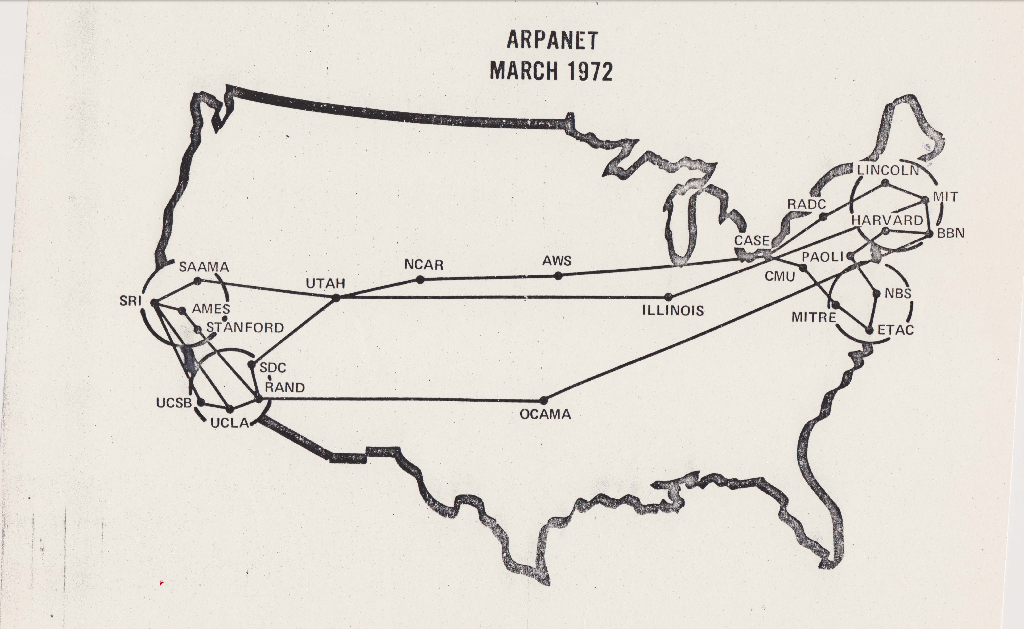
\includegraphics[width=0.5\linewidth]{images/arpanet_1972.png}
        \caption{Ferris the Crab \cite{arpanet}}
    \end{figure}

    \enote{
        \item Many modern devices used today are using the internet to communicate with each other
        \item A foundation for this can be found when looking at the ARPANET
        \item ARPANET: A packet-switching network deployed in the US
        \begin{enumerate}
            \item One of the first networks to implement the TCP/IP protocol suite
            \item Evolved into the Internet as we know it today
        \end{enumerate}
    }
\end{frame}
